\documentclass[a4paper]{article}
\usepackage[english]{babel}
\usepackage[utf8]{inputenc}
\usepackage{fancyhdr}
\usepackage{hyperref}
\usepackage{amsmath,amsfonts,amssymb,amsthm}
\usepackage[a4paper, bottom=1.3in, top=1.3in, right=1in, left=1in]{geometry}
\usepackage[usenames,dvipsnames]{xcolor}
\usepackage[lined,boxed]{algorithm2e}
\usepackage{natbib}
\usepackage{dsfont}
\usepackage{tikz}
\usetikzlibrary{calc}
\definecolor{amaranth}{rgb}{0.9, 0.17, 0.31}
\newcommand{\rcol}[1]{{\color{amaranth}#1}}

\usepackage{todonotes}
\newcommand{\todomp}[1]{\todo[color=Green!10, inline]{\small MP: #1}}
\newcommand{\todompout}[1]{\todo[color=Green!10]{\scriptsize MP: #1}}

\newcommand{\wh}[1]{\widehat{#1}}
\newcommand{\wt}[1]{\widetilde{#1}}
\newcommand{\transp}{\intercal}

%%%%%%%%%%%%%%%%%%%%%%%%%%%%%%%%%%%%%%%%%%%
% Insert your name here
\newcommand{\fullname}{Raphael Reme}
%%%%%%%%%%%%%%%%%%%%%%%%%%%%%%%%%%%%%%%%%%%

\newcommand{\lecture}[3]{
   \pagestyle{myheadings}
   \thispagestyle{plain}
   \newpage
   \setcounter{page}{1}
   \noindent
   \begin{center}
   \framebox{
      \vbox{\vspace{2mm}
              \hbox to .97\textwidth { {\bf MVA: Reinforcement Learning (2020/2021) \hfill Homework 4} }
       \vspace{6mm}
       \hbox to .97\textwidth { {\Large \hfill #1 \hfill } }
       \vspace{6mm}
       \hbox to .97\textwidth { {Lecturers: \it A. Lazaric, M. Pirotta  \hfill {{\footnotesize(
           January 9, 2020
        %    \today
           )}}} }
      \vspace{2mm}}
   }
   \end{center}
   Solution by {\color{amaranth}\fullname}
   \markboth{#1}{#1}
   \vspace*{4mm}
}


\DeclareMathOperator*{\argmax}{\arg\,\max}
\DeclareMathOperator*{\argmin}{\arg\,\min}
\DeclareMathOperator*{\arginf}{\arg\,\inf}


\setlength{\parindent}{0cm}
\begin{document}
\lecture{Model Selection for Contextual Bandit}{4}


\pagestyle{fancy}
\fancyhf{}
\rhead{Full name: {\color{amaranth}\fullname}}
\lhead{Model Selection for Contextual Bandit}
\cfoot{\thepage}

\textbf{Instructions}
\begin{itemize}
   \item The deadline is \textbf{February 5, 2021. 23h00}
   \item By doing this homework you agree to the \emph{late day policy, collaboration and misconduct rules} reported on \href{https://piazza.com/class/kf86owfvi2u2lg?cid=8}{Piazza}.
   \item \textbf{Mysterious or unsupported answers will not receive full credit}.
         A correct answer, unsupported by calculations, explanation, or algebraic work will receive no credit; an incorrect answer supported by substantially correct calculations and explanations might still receive partial credit.
   \item Answers should be provided in \textbf{English}.
\end{itemize}


\section{Model Selection}
In this homework, we look into the problem of model selection for bandit. For example,
\begin{itemize}
   \item Optimizing the exploration rate in an $\epsilon$-greedy algorithm
   \item Learning the most effective representation of a problem (e.g., UCB v. LinUCB, or selection among multiple linear representations)
\end{itemize}
These are just two examples of possible applications.

In general, we assume that we are given a set of $M$ bandit algorithms. We aim to design a meta algorithm (or \emph{master algorithm}) which selects at each round which base algorithm to play. The goal is to ensure that the performance of the master is not far away from the best base algorithm had it been run separately. Denote by $R_i(T)$ the regret bound of base algorithm $i$, the objective is to design a master algorithm having regret bound $\wt{O}(poly(M) R_{i^\star}(T))$, where $R_{i^\star}(T) = \min_i R_i(T)$.
This problem has received a lot of attention over the years~\citep{AgarwalDKLS12,AgarwalLNS17,SinglaH017}, with a surge of interest this year~\citep{AbbasiYadkori2020regrebalancing,PacchianoPA0ZLS20,pacchiano2020regret}.

\vspace{.2in}
While this idea applies to many scenarios, we consider the problem of selecting a representation for LinUCB.
We start reviewing the setting of linear contextual bandit.
At each round $t$, the algorithm receives a context $x_t \in \mathcal{X}$ (we assume the contexts are drawn i.i.d.\ from $\mathcal{X}$) and needs to select an action $a_t \in \mathcal{A}$ to play (we assume $\mathcal{A}$ is finite).
The reward associated to a context-action pair ($x,a$) is a linear function of a set of features in $\mathbb{R}^d$: $r(x,a) = \langle \phi(x,a), \theta^\star \rangle$. The vector $\theta^\star \in \mathbb{R}^d$ is unknown and the observed reward at time $t$ is a noisy version of the true reward: $r_t(x,a) = r(x,a) + \eta_t$ with $\eta_t$ being a conditionally zero mean $\sigma$-subgaussian random variable. The objective is to control the pseudo-regret: $R(T) = \sum_{t=1}^T \langle \phi(x, a^\star) - \phi(x,a_t), \theta^\star \rangle$. LinUCB algorithm suffers a regret at most $\wt{O}(\log(\det(\Sigma_t)/delta) \sqrt{t}) \leq \wt{O}(d\sqrt{t})$ for any $t \leq T$, where $\Sigma_t = \sum_{i=1}^t  \phi(x_i, a_i) \phi(x_i, a_i)^\top + \lambda I$ is the $(\lambda>0)$-regularized design matrix.

We now assume that the mapping $\phi$ is unknown but we have access to a set of candidates $F = (f_i)_{i \in [M]}$. We can instantiate a version of LinUCB for each representation $f \in F$. Denote by $B_i = LinUCB(f_i)$.
The new interaction loop is as follows. At each round $t$, the master observes a context $x_t$ and needs to select the base algorithm $B_t$ to play among the $M$ variants of LinUCB. $B_t$ is executed, i.e., $B_t$ selects the action $a_t$ to play and a reward $r_t(x_t,a_t) = \langle \phi(x,a), \theta^\star \rangle + \eta_t$ is observed. The master and $B_t$ are updated using the observed reward.
It is common to assume that at least one mapping is realizable
\[
   \exists f^\star \in F, \omega ~~:~~ \forall x,a, ~ r(s,a) = \langle \phi(x,a), \theta^\star \rangle =
   \langle f^\star(x,a), \omega \rangle
\]


\vspace{.2in}
We provided an initial code implementing a linear representation and a bandit problem. The goal is to investigate the approach in the paper~\citep{pacchiano2020regret} and implement their algorithm (Algorithm 1) in this setting.

You can play with the code to test your implementation. We provide a simple entry point in file \texttt{main\_simple.py} to test your implementation on small problems.

Consider the following setting for the final experiment (already implemented in the file \texttt{main\_final.py}).
We consider a finite set of contexts and actions: $|\mathcal{X}| = 200$, $|\mathcal{A}|=20$.
Let $|F| = 8$ and $f_8 = f^\star$ with $d_8 = d^\star = 20$ (i.e., the realizable representation). The others are such that
\begin{itemize}
   \item $f_1, f_2, f_3$ are nested representations of $f^\star$ with size $d_1 = 5$, $d_2 = 10$ and $d_3=25$ obtained by selecting the first $d_i$ features when $d_i < d^\star$ and padding random features when $d_i > d^\star$.
   \item $f_4, f_5, f_6, f_7$ are randomly generated feature of dimension $3, 7, 16, 30$.
\end{itemize}
Let $T=50000$, $\sigma = 0.3$, $\delta = 0.01$ and $\lambda=1$. Remember to average the regret over multiple runs.

Questions:
\begin{enumerate}
   \item Start from implementing LinUCB (a.k.a.\ OFUL). Use the slides or any other material as reference for the implementation (e.g., Section 6.1 in~\citep{pacchiano2020regret}). Suggestion: use Sherman–Morrison formula for a more efficient implementation.
   \item Understand the ``Regret Bound Balancing and Elimination Algorithm'' (RegBalAlg) in~\citep{pacchiano2020regret} (Algorithm 1).

         \tikz{
            \node[text width=0.9\textwidth, color=red] at (0,0) {
               \textbf{!} It's a long document, focus only on the parts relevant for the homework. Section 4 should be enough for implementing the algorithm. Clearly, previous sections are necessary to better understand the setting and the notation.
            };
         }

         \begin{enumerate}
            \item Could you briefly explain the idea behind the algorithm?
            \item Could you explain the elimination condition? What does the set $\mathcal{W}$ contain?
         \end{enumerate}
   \item Implement the algorithm ``Regret Bound Balancing and Elimination Algorithm'' (RegBalAlg) for the mentioned problem (see provided code).
         \begin{enumerate}
            \item Compare the RegBalAlg algorithm versus LinUCB on each representation (i.e., $B_i$ for $i \in [M]$). Report the a picture with the pseudo regret of each algorithm.
            \item What upper-bound did you use for implementing RegBalAlg?
            \item Is any representation eliminated? Is the optimal representation the only not eliminated? Try to explain what you observed.
            \item Plot the regret of RegBalAlg and the one of the optimal representation. If you see a sudden change in the regret of RegBalAlg, could you explain why this happens?
         \end{enumerate}
\end{enumerate}

\subsection*{Answers}
\subsubsection*{2.a}
The idea of the algorithm is to use several learners to solve the problem. Each learner is able to compute a bound
of the regret it will cause, given the number of times it is played. The key idea is that with only well-specified learners (learners that
respect this bound) and a specific playing order for learners, the total regret is bounded by the number of learners we have times the best
learner's bound for regret, assuming that we only played this learner.

In order to have this bound, the playing order of learners is so that each learner has caused a roughly equal presumed regret bound given
the number of times it has been played. The algorithm therefore choose to play at each round the learner that is responsible
for the smallest presumed regret bound (given the number of times it has been played at this round).

But of course, learners are not always well-specified. To solve this issue, the algorithm eliminate learners that are miss-specified. They use a
simple equation at each round, that if verified ensure that a given learner is miss-specified with high probability and should therefore
be eliminated. (This equation is build in a similar way than the one we had in the previous homework for best arm identification!)

\subsubsection*{2.b}

\begin{equation*}
   W = \{i \in [M]: \forall t \in [T], \; \text{Reg}_i(t) \le R_i(n_i(t))\}
\end{equation*}

$W$ is the set of well-specified learners: The learners so that the regret they have caused ($\text{Reg}_i(t)$) is smaller than the presumed
regret bound of the learner ($R_i(n_i(t))$, with $n_i(t)$ the number of times this learner have been played at round $t$.)

They showed that if a learner $i$ is well-specified then we have with probability $1 - \delta$:
\begin{equation*}
   \frac{U_i(t)}{n_i(t)} - c\sqrt{f_i(t, \delta)} \le \mu^\star \le \frac{U_i(t)}{n_i(t)} + c\sqrt{f_i(t, \delta)} + \frac{R_i(n_i(t))}{n_i(t)}
\end{equation*}
With $U_i$ the sum of the rewards obtained playing the learner $i$, and $f_i(t, \delta) = \frac{1}{n_i(t)} \ln(M \ln\frac{n_i(t)}{\delta})$.
(Note that the left part is always verified even if the learner is miss-specified)

The idea is then to check if it exists $j$ such that
\begin{equation*}
   \frac{U_i(t)}{n_i(t)} + c\sqrt{f_i(t, \delta)} + \frac{R_i(n_i(t))}{n_i(t)} <  \frac{U_j(t)}{n_j(t)} - c\sqrt{f_j(t, \delta)} \;\;\;\;\;\; (\le \mu^\star)
\end{equation*}
In this case, $i$ cannot verify the previous equation and thus is not well specified. The algorithm therefore removes $i$.

\subsubsection*{3.a}


\begin{figure}[h!]
   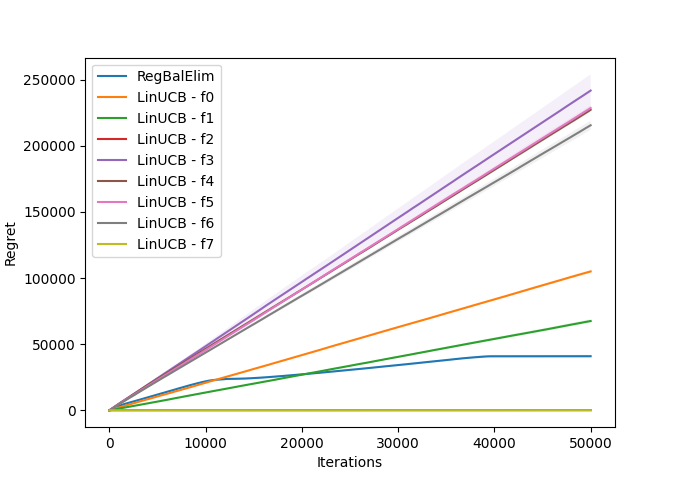
\includegraphics[width=0.8\linewidth]{images/regret}
   \caption{Pseudo-Regret with 8 different LinUCB and the RegBalAlg}
   \label{fig:regret}
\end{figure}

One can see that for LinUCB the representation plays a huge role in the regret the algorithm suffers. The regret is linear but the slope
is not the same, for the true representation the slope is much smaller.

On the other hand, the RegBalAlg is able to select the best representations after some iterations and improves over time. After around 40 000
iterations, we are suffering a similar immediate regret than with the good representation.

\subsubsection*{3.b}

I used the upperbound found in the annexe of~\citep{pacchiano2020regret} (p.54):

\begin{equation*}
   r_t \le 2 \beta_t ||a_t||_{\Sigma_t^{-1}}
\end{equation*}

With $r_t$ the immediate regret at round $t$. This quantity is easily computable as we already have to compute $\beta_t ||a_t||_{\Sigma_t^{-1}}$
in the LinUCB algorithm. Therefore each LinUCB learner can compute its presumed regret bound. It's also a tighter bound than the one they
proposed in the article.

Note: With the bound they proposed it does not work well. It's possible that, because I used a bound over $\beta_t$ rather than
$\beta_t$ itself (From the slides or equation $(14)$), I have to compensate and be tighter in my presumed regret bound.


\subsubsection*{3.c}
The algorithm eliminate all the representations except the true one (f7) and the best other one (f2).

It does not eliminate the f2 representation because it yields very similar results as the true one. The real explanation is that
the two representations are totally equivalent: The f2 representation is a copy of the f7 one with 5 more dimensions that are unused. (I added
some code to show it.) And therefore the LinUCB with f2 is as efficient as the one on f7.

\subsubsection*{3.d}

\begin{figure}[h!]
   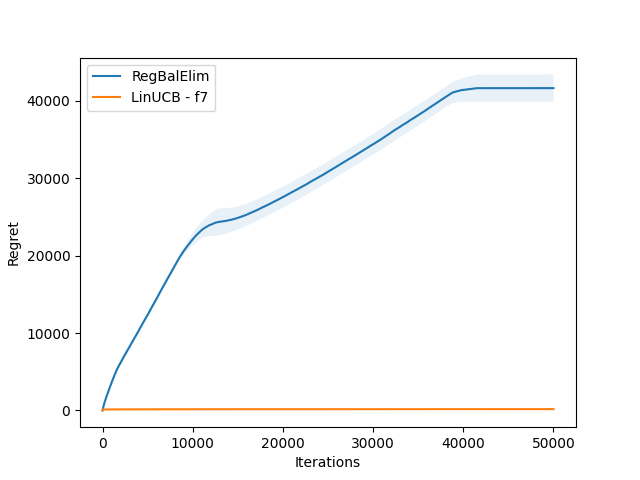
\includegraphics[width=0.8\linewidth]{images/regret2}
   \caption{Pseudo-Regret for RegBalAlg and LinUCB on the best representation}
   \label{fig:regret2}
\end{figure}

We can see sudden changes in the regret of RegBalAlg, an explanation is that at each change the algorithm has stopped using some of the wrong
representations (which occurs around their elimination), and therefore has become much more efficient.

The change around 10 000 iterations corresponds to the eliminitation of representations f5 and f1. And the change around 40 000 iterations
corresponds to the eliminitation of representation f6. (The other representations are eliminated sooner)


\bibliographystyle{plainnat}
\bibliography{bibliography}
\end{document}
